\section{Caracteriza\c{c}\~{a}o microestrutural}

\label{sec:micros}

\subsection{Microscopia óptica}

A Figura \ref{fig:temperada} mostra a microestrutura da amostra austenitizada a 880 °C e temperada à temperatura ambiente no dilatômetro Bähr. Além dos nódulos de grafita do ferro fundido, nota-se a presença de martensita em morfologia de placas, colorida em tons azulados castanhos, e áreas brancas presentes entre as placas de martensita. Essa tonalidade branca corresponde à resposta da fase austenita quando exposta ao reagente Beraha.

\begin{figure}
	\includegraphics[width=10cm]{img/micrografias/MO/temperada/1000x-1.pdf}
	\caption{Imagens obtidas por microscopia óptica da amostra temperada a temperatura ambiente. Aumento de 1000x.}
	\label{fig:temperada}
\end{figure}

As Figuras \ref{fig:TT140TP300}a e \ref{fig:TT140TP300}b mostram a microestrutura da amostra temperada a 140 °C e particionada a 300 °C. Em baixo aumento (100x) é possível observar extensas áreas brancas, associadas a regiões com maior predominância de austenita retida. Por sua vez, a localização da austenita é relacionada aos contornos de célula eutética formados durante a solidificação. Devido à segregação de elementos gamagênicos para estas regiões, espera-se que uma quantidade maior de austenita retida seja observada nesses locais. Esse mesmo comportamento é observados nas demais amostras tratadas termicamente.

\begin{figure}
	\subfloat[]{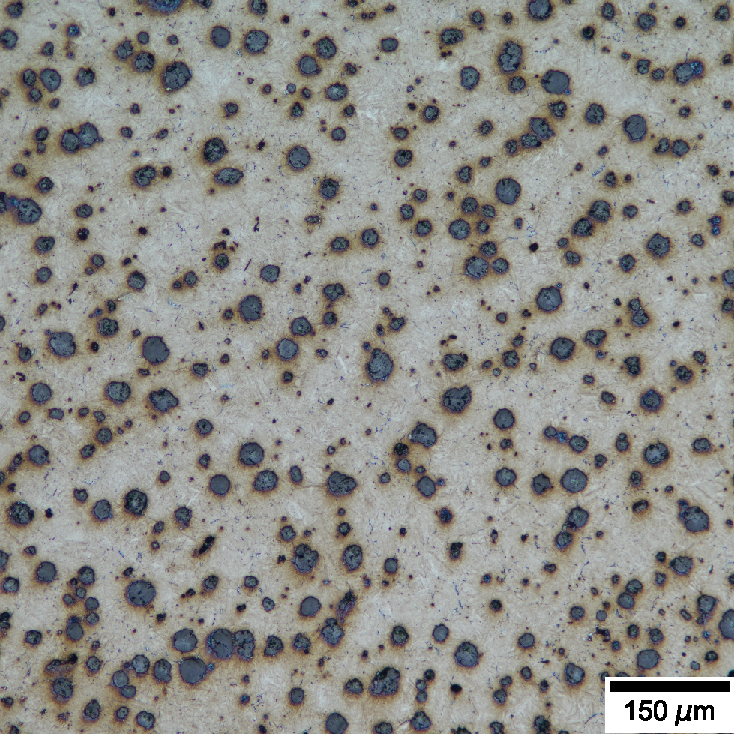
\includegraphics[width=10cm]{img/micrografias/MO/TT140TP300/100x-1.pdf}}
	\vspace{0pt}
	\subfloat[]{\includegraphics[width=10cm]{img/micrografias/MO/TT140TP300/1000x-1.pdf}}
	\caption{Imagens obtidas por microscopia óptica da amostra temperada a 140 °C e particionada a 300 °C. (a) Aumento de 100x. (b) Aumento de 1000x.}
	\label{fig:TT140TP300}
\end{figure}

Em maiores aumentos (Figura \ref{fig:TT140TP300}b) nota-se a presença de placas mais grosseiras, correlatas a placas de martensita formadas durante a etapa de têmpera do processo T\&P, e um produto muito mais refinado, associado ao produto isotérmico formado durante a partição. A morfologia desse produto é característica da bainita isenta de carbonetos, ou ausferrita, observada nos ferros fundidos nodulares austemperados. Adicionalmente, constata-se que as regiões de austenita não se limitam somente aos contornos de célula eutética, mas se estendem também às regiões entrecortadas pelos feixes de ausferrita e placas de martensita.

Nas Figuras \ref{fig:TT170TP300x1000} e \ref{fig:TT200TP300x1000} são mostradas as microestruturas das amostras também particionadas a 300 °C, mas temperadas nas temperaturas de 170 e 200 °C, respectivamente. Observa-se que, embora os resultados de dilatometria e de difração de raios X apontem a existência de menores quantidades de placas martensita do que na amostra temperada a 140 °C (Figura \ref{fig:TT140TP300}b), essa diferença é pouco perceptível na análise microestrutural. Nota-se uma nítida diferença na dimensão longitudinal dos feixes de ausferrita, aparentando ser mais longos quanto maior a temperatura de têmpera. Isso é condizente com a maior repartição do espaço produzida em menores temperaturas de têmpera, tendo em vista as maiores quantidades produzidas de martensita.

\begin{figure}
	\includegraphics[width=10cm]{img/micrografias/MO/TT170TP300/1000x-2.pdf}
	\caption{Imagem obtida por microscopia óptica da amostra temperada a 170 °C e particionada a 300 °C. Aumento de 1000x.}
	\label{fig:TT170TP300x1000}
\end{figure}

\begin{figure}
	\includegraphics[width=10cm]{img/micrografias/MO/TT200TP300/1000x-2.pdf}
	\caption{Imagem obtida por microscopia óptica da amostra temperada a 200 °C e particionada a 300 °C. Aumento de 1000x.}
	\label{fig:TT200TP300x1000}
\end{figure}

Além da mudança da escala dos feixes de ausferrita, a alteração da temperatura de têmpera não parece ter qualquer outro efeito na morfologia do produto isotérmico. Por outro lado, é razoável esperar que mudanças na morfologia da ausferrita sejam observadas para diferentes condições de temperaturas de partição.

As Figuras \ref{fig:TT170TP200x1000} a \ref{fig:TT170TP450x1000} mostram as microestruturas das amostras temperadas a 170 °C e particionadas a 200, 250, 375 e 450 °C (a amostra particionada a 300 °C é mostrada na Figura \ref{fig:TT200TP300x1000}). Para estas condições de tratamento térmico não são esperadas diferenças nas quantidades de placas de martensita formadas durante a etapa de têmpera. Por outro lado, diferenças significativas na morfologia do produto isotérmico são observadas.

\begin{figure}
	\includegraphics[width=10cm]{img/micrografias/MO/TT170TP200/1000x-2.pdf}
	\caption{Imagem obtida por microscopia óptica da amostra temperada a 170 °C e particionada a 200 °C. Aumento de 1000x.}
	\label{fig:TT170TP200x1000}
\end{figure}

\begin{figure}
	\includegraphics[width=10cm]{img/micrografias/MO/TT170TP250/1000x-2.pdf}
	\caption{Imagem obtida por microscopia óptica da amostra temperada a 170 °C e particionada a 250 °C. Aumento de 1000x.}
	\label{fig:TT170TP250x1000}
\end{figure}

\begin{figure}
	\includegraphics[width=10cm]{img/micrografias/MO/TT170TP375/1000x-1.pdf}
	\caption{Imagem obtida por microscopia óptica da amostra temperada a 170 °C e particionada a 375 °C. Aumento de 1000x.}
	\label{fig:TT170TP375x1000}
\end{figure}

\begin{figure}
	\includegraphics[width=10cm]{img/micrografias/MO/TT170TP450/1000x-1.pdf}
	\caption{Imagem obtida por microscopia óptica da amostra temperada a 170 °C e particionada a 450 °C. Aumento de 1000x.}
	\label{fig:TT170TP450x1000}
\end{figure}

Na amostra particionada na temperatura de 200 °C (Figura \ref{fig:TT170TP200x1000}) as setas vermelhas indicam a presença de ferrita pró-eutetóide formada durante o resfriamento da temperatura de austenitização até a temperatura de têmpera. A caracterização nesta condição foi feita em uma amostra tratada na linha XTMS, na qual taxas de resfriamento menores foram conseguidas. Consequentemente, permitiu-se a formação de pequenas quantidades de ferrita durante o resfriamento, devido à reduzida temperabilidade do material. Fora esse detalhe, não se observa produtos pró-bainíticos aciculares, como fora observado na condição de partição a 300 °C. De fato, a amostra particionada nesta temperatura se assemelha à obtida na condição temperada (Figura \ref{fig:temperada}).

A microestrutura da amostra particionada a 250 °C (Figura \ref{fig:TT170TP250x1000}) apresenta extensas regiões de austenita. No entanto, tendo em vista a estabilidade da austenita produzida nesta condição (Ms = 77 °C), é possível que estas regiões na verdade correspondam a uma mistura de austenita e martensita fresca produzida durante o resfriamento final. Observam-se também placas de martensita produzida durante a etapa de têmpera e finos produtos aciculares associados novamente à reação bainítica. Em comparação às imagens das amostras particionadas a 300 °C, nota-se que o produto produzido a 250 °C é mais refinado e é de difícil interpretação apenas por microscopia óptica.

Na amostra tratada isotermicamente a 375 °C (Figura \ref{fig:TT170TP375x1000}) o produto isotérmico é semelhante ao observado a 300 °C, mas apresenta-se na forma de ripas mais grosseiras de ferrita. As regiões brancas nessa amostra são interpretadas sendo puramente austenita estabilizada pelo carbono. Nas amostras particionadas a 450 °C (Figura \ref{fig:TT170TP450x1000}), embora não tenham sido quantificados frações volumétricas de austenita pela difração de raios X, observam-se regiões brancas nas regiões de contornos de célula eutética (setas vermelhas). A natureza desse produto, no entanto, não pode ser determinada nas magnificações permitidas pelo microscópio óptico.

\subsection{Microscopia eletrônica}

A Figura \ref{fig:temperadax25k} mostra a imagem da microestrutura da amostra austenitizada a 880 °C e temperada à temperatura ambiente obtida por microscopia eletrônica de varredura (MEV). As Figuras \ref{fig:TT170TP200x10k} a \ref{fig:TT170TP450x25k} mostram as imagens microestruturas das amostras temperadas a 170 °C e particionadas entre 200 e 450 °C também obtidas por MEV. Nas Figura \ref{fig:TT170TP250x10k} a \ref{fig:TT170TP375x10k} as setas em vermelho indicam a ferrita bainítica formada durante a etapa de partição e as setas em azul indicam as placas de martensita formadas durante a etapa de têmpera. A análise nas magnificações permitidas pelo MEV mostram claramente as diferenças entre as escalas do microconstituinte bainítico formado nas amostras particionadas a 250, 300, 375 e 450 °C.

%temperada
\begin{figure}
	\includegraphics[width=10cm]{img/micrografias/MEV/temperada/25k-1.pdf}
	\caption{Imagem obtida por microscopia eletrônica de varredura da amostra temperada à temperatura ambiente. Aumento de 25kx.}
	\label{fig:temperadax25k}
\end{figure}

%200 °C
\begin{figure}
	\includegraphics[width=10cm]{img/micrografias/MEV/TT170TP200/10k-1.pdf}
	\caption{Imagem obtida por microscopia eletrônica de varredura da amostra temperada a 170 °C e particionada a 200 °C. Aumento de 10kx.}
	\label{fig:TT170TP200x10k}
\end{figure}

\begin{figure}
	\includegraphics[width=10cm]{img/micrografias/MEV/TT170TP200/25k-1.pdf}
	\caption{Imagem obtida por microscopia eletrônica de varredura da amostra temperada a 170 °C e particionada a 200 °C. Aumento de 25kx.}
	\label{fig:TT170TP200x25k}
\end{figure}

%250 °C
\begin{figure}
	\includegraphics[width=10cm]{img/micrografias/MEV/TT170TP250/10k-1.pdf}
	\caption{Imagem obtida por microscopia eletrônica de varredura da amostra temperada a 170 °C e particionada a 250 °C. Aumento de 10kx.}
	\label{fig:TT170TP250x10k}
\end{figure}

\begin{figure}
	\includegraphics[width=10cm]{img/micrografias/MEV/TT170TP250/50k-4.pdf}
	\caption{Imagem obtida por microscopia eletrônica de varredura da amostra temperada a 170 °C e particionada a 250 °C. Aumento de 50kx.}
	\label{fig:TT170TP250x50k}
\end{figure}

%300 °C
\begin{figure}
	\includegraphics[width=10cm]{img/micrografias/MEV/TT170TP300/10k-1.pdf}
	\caption{Imagem obtida por microscopia eletrônica de varredura da amostra temperada a 170 °C e particionada a 300 °C. Aumento de 10kx.}
	\label{fig:TT170TP300x10k}
\end{figure}

%375 °C
\begin{figure}
	\includegraphics[width=10cm]{img/micrografias/MEV/TT170TP375/10k-2.pdf}
	\caption{Imagem obtida por microscopia eletrônica de varredura da amostra temperada a 170 °C e particionada a 375 °C. Aumento de 10kx.}
	\label{fig:TT170TP375x10k}
\end{figure}

%450 °C
\begin{figure}
	\includegraphics[width=10cm]{img/micrografias/MEV/TT170TP450/10k-8.pdf}
	\caption{Imagem obtida por microscopia eletrônica de varredura da amostra temperada a 170 °C e particionada a 450 °C. Aumento de 10kx.}
	\label{fig:TT170TP450x10k}
\end{figure}

\begin{figure}
	\includegraphics[width=10cm]{img/micrografias/MEV/TT170TP450/25k-1.pdf}
	\caption{Imagem obtida por microscopia eletrônica de varredura da amostra temperada a 170 °C e particionada a 450 °C. Aumento de 25kx.}
	\label{fig:TT170TP450x25k}
\end{figure}

A análise da microestrutura da amostra particionada a 200 °C (Figura \ref{fig:TT170TP200x10k}) revela apenas a presença de placas de martensita, como já apontado nos resultados anteriores. No entanto, nota-se uma diferença no padrão de ataque da amostra tratada nesta condição da amostra temperada à temperatura ambiente (Figura \ref{fig:temperadax25k}). Na amostra temperada e particionada a martensita parece ter sido consumida não-uniformemente pelo reagente durante o ataque metalográfico. Por outro lado, o ataque aplicado à amostra temperada produziu superfícies lisas em baixo relevo. A análise em maior magnificação da amostra T\&P é mostrada na Figura \ref{fig:TT170TP200x25k}. Observa-se que o padrão de ataque desenvolvido na martensita revela pequenos alvéolos alinhados entre si no interior das placas de martensita. Padrão semelhante é observado nas placas de martensita particionadas nas demais condições.

Em um primeiro momento, chega-se a especular que estes alvéolos poderiam se tratar de carbonetos de transição do revenimento da martensita. No entanto, a literatura é clara em dizer que os carbonetos de revenimento precipitam-se inclinados em diferentes ângulos em relação ao eixo central da placa de martensita. %citation needed
Dessa forma, teoriza-se que o padrão de ataque produzido é decorrente de fenômenos de redistribuição de carbono no interior da própria placa de martensita, quando não da partição de carbono da martensita para a austenita.

Na amostra particionada a 250 °C observa-se que a fração da fase acicular é menor do que à obtida nas amostras tratadas a 300 e 375 °C. Como pode ser observado na Figura \ref{fig:TT170TP250x50k}, as regiões em alto relevo correspondentes aos espaços não transformados entre as agulhas de ferrita bainítica e as placas de martensita formam blocos poligonais. O padrão de ataque não permite concluir, no entanto, se essas regiões foram ou não parcialmente transformadas em martensita durante o resfriamento final.

Nas amostra particionada a 375 °C também são observados blocos poligonais não transformados (Figura \ref{fig:TT170TP300x10k}). Nesse caso, o compilados dos resultados apresentados até o momento permite afirmar que estas regiões consistem de austenita estabilizada pelo seu enriquecimento em carbono. A repartição do espaço pelo produto bainítico nesta condição é menor do que na amostra particionada a 300 °C, na qual são observadas ilhas de austenita ``mais finas'', tal qual o produto bainítico.

Por sua vez, na amostra particionada a 450 °C é observada uma fina dispersão de precipitados ao longo de todo o material (Figura \ref{fig:TT170TP450x10k}), provavelmente provenientes do segundo estágio da reação bainítica e do revenimento da martensita. A Figura \ref{fig:TT170TP450x25k} foi obtida sobre uma região análoga à área branca observada na imagem de microscopia óptica na Figura \ref{fig:TT170TP450x1000}. O padrão de ataque revela uma microestrutura que se assemelha à ripas bastante grosseiras de ausferrita, sendo as regiões em alto relevo correspondentes a austenita não transformada. Embora austenita não tenha sido quantificada pelos resultados de raios X, é provável que a austenita observada se apresente em tão pequena quantidade que os picos de difração desta fase tenham se confundido com o ruído de fundo do difratograma.